\chapter{热与绝热}\label{ch:g5:heat-and-insulation}

为什么金属滑梯摸起来冰凉，旁边的木长椅却不会？
这个谜团从本书第一年起就一直伴随着我们。
今天，它的答案揭晓了——连同保温瓶的秘密、
双层窗户的道理，以及蓬起羽毛过冬的麻雀。关键在于
不再追问东西\emph{摸起来}怎样，而要开始追踪\omterm{def:g5:heat-and-insulation:heat}{热量}
\emph{流向}何方。

\section{热量在流动}

\begin{definition}[热量]\label{def:g5:heat-and-insulation:heat}
\emph{热量}\index{热量}是\omterm{def:g5:everyday-energy:energy}{能量}从较热的物体
向较冷的物体转移。汤把热量传给勺子，暖气片把热量传给
房间，你的手把热量传给雪球。热量并不是藏在热物体里的
某种物质，它是一种\emph{流动}，并且总
有方向。
\end{definition}

\begin{proposition}[热量向低处流]\label{prop:g5:heat-and-insulation:downhill}
\omterm{def:g5:heat-and-insulation:heat}{热量}自然总是从\omterm{def:g3:temperature-thermometers:temperature}{温度}较高的物体流向\omterm{def:g3:temperature-thermometers:temperature}{温度}较低的
物体，绝不会反向。只要两者\omterm{def:g3:temperature-thermometers:temperature}{温度}不同，流动就持续，
而当两者\omterm{def:g3:temperature-thermometers:temperature}{温度}趋于一致时，流动便逐渐消失。若让
冷热相邻的两个物体接触足够长的时间，它们
最终会达到同一\omterm{def:g3:temperature-thermometers:temperature}{温度}。
\end{proposition}

\begin{example}[判断热量的方向]\label{ex:g5:heat-and-insulation:direction}
茶中的小勺变热了：\omterm{def:g5:heat-and-insulation:heat}{热量}从茶 $\to$ 勺子。
加了冰块的柠檬水变凉了——请注意！并没有
名为“冷”的东西流进去：\omterm{def:g5:heat-and-insulation:heat}{热量}是从柠檬水\emph{流入
冰块}，使冰块\omterm{def:g2:ice-water-steam:meltfreeze}{熔化}。冷并不是一种流动，它只是我们给
失去\omterm{def:g5:heat-and-insulation:heat}{热量}一方起的名字。物理书上都写“饮料失去了\omterm{def:g5:heat-and-insulation:heat}{热量}”，
从不写“饮料得到了冷”。
\end{example}

\begin{omfigure}
\begin{tikzpicture}[scale=0.85]
  \draw[thick] (0.6,0.4) rectangle (3.0,1.9);
  \node[font=\small] at (1.8,1.15) {热汤};
  \draw[thick] (7.8,0.4) rectangle (10.2,1.9);
  \node[font=\small] at (9.0,1.15) {凉空气};
  \draw[-Stealth, line width=3pt, omThm] (3.3,1.15) -- (7.5,1.15);
  \node[above, font=\small, omThm] at (5.4,1.4)
    {热量由热 $\to$ 冷流动};
  \node[below, font=\small] at (5.4,0.0)
    {直到两者温度相同才停止};
\end{tikzpicture}

{\small 每个厨房、每个冬天都遵循同一条规律：\omterm{def:g5:heat-and-insulation:heat}{热量}向低处流，从热到冷，
直到“坡”消失为止。}
\end{omfigure}

\section{快车道与慢车道}

\begin{definition}[热的良导体与热的不良导体]\label{def:g5:heat-and-insulation:conductors}
不同物质让\omterm{def:g5:heat-and-insulation:heat}{热量}通过的快慢相差悬殊。
\emph{热的良导体}\index{热的良导体}是快车道，
金属尤其如此。\emph{热的不良导体}\index{热的不良导体}则是
慢车道：木头、羊毛、塑料、羽毛都是；而冠军是
\emph{静止的\omterm{def:g2:air-around-us:air}{空气}}，只要它被困住、无法对流。（这两个词是
有意借用电学中的\omterm{def:g4:conductors-insulators:conductor}{导体}与\omterm{def:g4:conductors-insulators:insulator}{绝缘体}；
这两类性质常常一致，但并非总是如此。）
\end{definition}

\begin{omfigure}
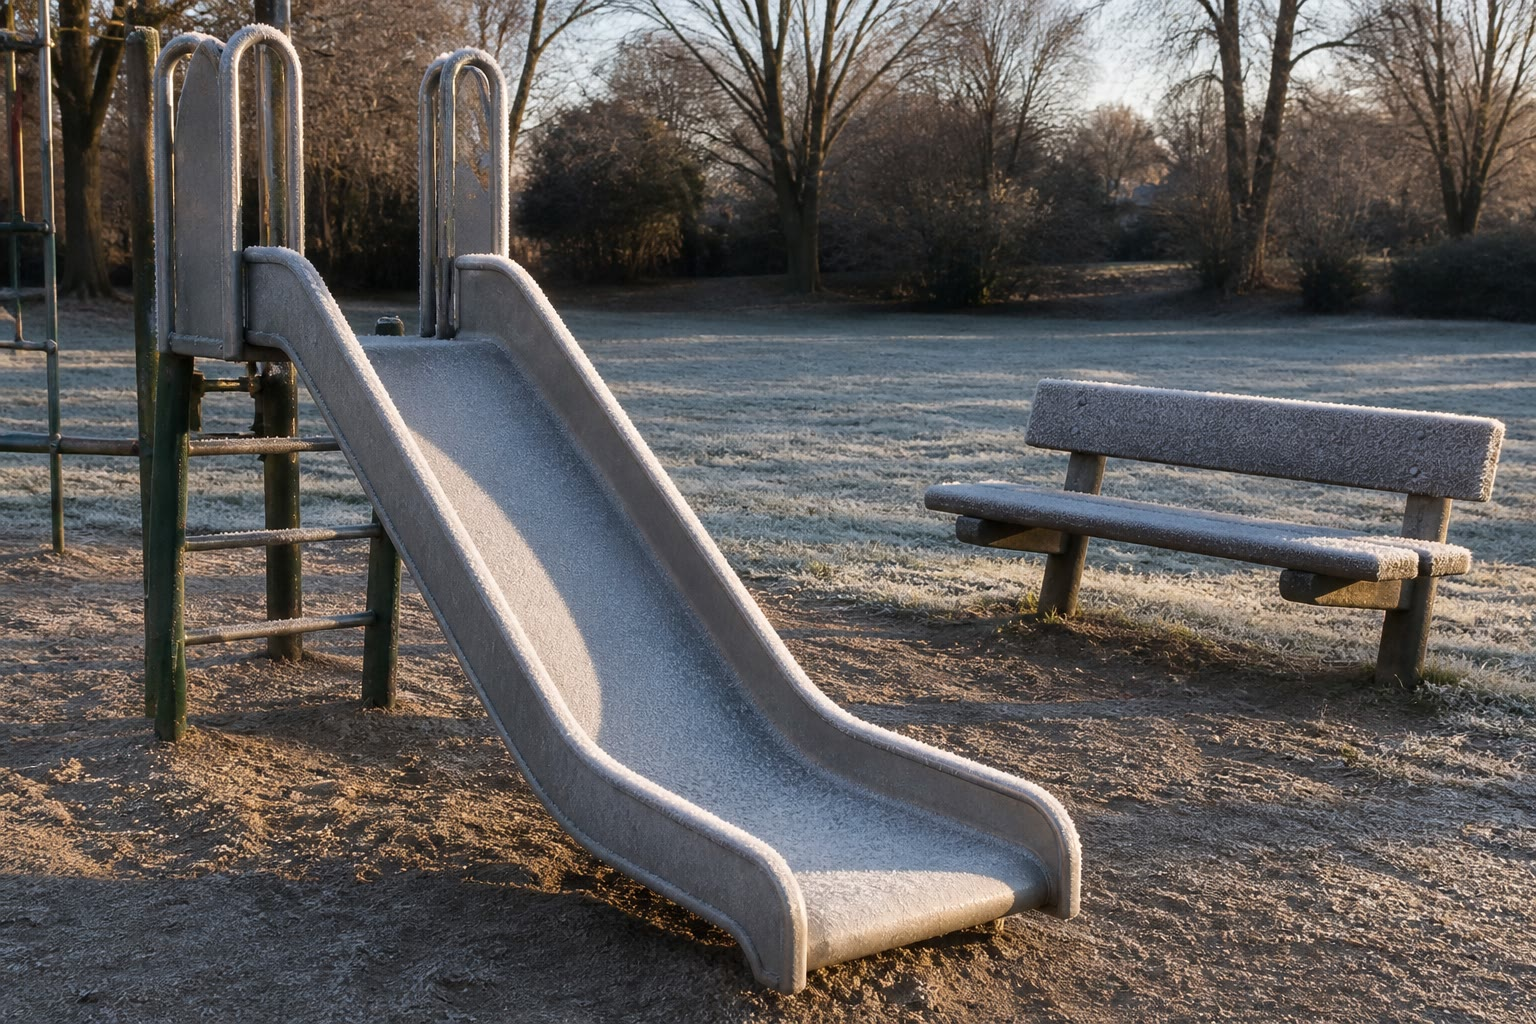
\includegraphics[width=0.58\linewidth]{images/book1/ai/g5-heat-frosty-slide.jpg}

{\small 霜冻的早晨，操场上：金属滑梯与木长椅在同一个夜晚处于相同的\omterm{def:g3:temperature-thermometers:temperature}{温度}——但只有其中一个会刺痛你的皮肤。}
\end{omfigure}

\begin{example}[滑梯之谜的解答]\label{ex:g5:heat-and-insulation:slide}
金属滑梯与木长椅整夜都处于同一个寒冷的
\omterm{def:g3:temperature-thermometers:temperature}{温度}——\omterm{def:g3:temperature-thermometers:temperature}{温度计}早已证实了这一点。摸一摸
它们：你的手比两者都暖，因此\omterm{def:g5:heat-and-insulation:heat}{热量}从你的手
流入每一个。但金属是快车道，它会迅速
带走你的\omterm{def:g5:heat-and-insulation:heat}{热量}，而这种\emph{迅速}的流失正是
“冰凉”的感觉所在。木头只缓缓带走你的\omterm{def:g5:heat-and-insulation:heat}{热量}：
几乎只是微凉。你的皮肤从来不是在\omterm{def:g2:measuring-length:measure}{测量}\omterm{def:g3:temperature-thermometers:temperature}{温度}，
它\omterm{def:g2:measuring-length:measure}{测量}的是自身\omterm{def:g5:heat-and-insulation:heat}{热量}散失的速度。谜团就此解开，耗时四年。
\end{example}

\begin{method}[冷却比赛]\label{met:g5:heat-and-insulation:race}
用数字看绝热如何取胜：
\begin{enumerate}
  \item 取两个相同的杯子，各倒入同样热的自来水
        （\emph{请大人帮忙，水温以手感温热为宜，不要沸腾}）；
  \item 用羊毛围巾把其中一个杯子厚厚地包起来，另一个不包；
  \item 把\omterm{def:g3:temperature-thermometers:temperature}{温度计}分别插入两个杯子，每隔五分钟记录一次两杯的\omterm{def:g3:temperature-thermometers:temperature}{温度}，
        共记录六次，并列成表格；
  \item 把两组记录画在同一张图上，画成两条折线，
        纵轴为\omterm{def:g3:temperature-thermometers:temperature}{温度}，横轴为时间。
\end{enumerate}
未包裹的杯子的曲线急剧下降，包裹后的杯子的曲线缓缓倾斜。
起点相同，房间也相同——羊毛让\omterm{def:g5:heat-and-insulation:heat}{热量}的出口变成了慢车道。
\end{method}

\begin{omfigure}
\begin{tikzpicture}
\begin{axis}[omaxis, width=10.5cm, height=5.6cm,
    xlabel={时间（分钟）}, ylabel={温度（\unit{\celsius}）},
    xtick={0,5,10,15,20,25,30}, ytick={20,30,40,50},
    ymin=15, ymax=55, xmin=-1, xmax=31]
  \addplot[very thick, omDef] coordinates
    {(0,50) (5,46.5) (10,43.5) (15,41) (20,39) (25,37.5) (30,36)};
  \addplot[very thick, omThm] coordinates
    {(0,50) (5,41) (10,34.5) (15,30) (20,27) (25,24.5) (30,23)};
  \node[right, font=\small, omDef] at (axis cs:24,39.5)
    {包裹羊毛};
  \node[right, font=\small, omThm] at (axis cs:19,25.5) {未包裹的杯子};
\end{axis}
\end{tikzpicture}

{\small 冷却赛跑，画成图：两杯 \qty{50}{\celsius}
的水放在 \qty{20}{\celsius} 的房间里。羊毛无法阻止\omterm{def:g5:heat-and-insulation:heat}{热量}
散失，但能把它减慢得很好。}
\end{omfigure}

\begin{remark}[保温只能减慢]\label{rem:g5:heat-and-insulation:onlyslows}
看看两条曲线的走向：都朝着房间的
\qty{20}{\celsius}。没有围巾，没有保温瓶，也没有冰屋的墙，能真正阻止
\omterm{def:g5:heat-and-insulation:heat}{热量}顺流而下的流动——保温只是让这条慢车道
变得更慢。这也是为什么雪人身上的外套（还记得他吗？）
延缓了他的融化，却没能救他：夏天的\omterm{def:g5:heat-and-insulation:heat}{热量}仍然
一点点渗进来。
\end{remark}

\section{困住空气的艺术}

\begin{example}[冬季工程]\label{ex:g5:heat-and-insulation:air}
你拥有的几乎每样保暖的东西，都是一台困住\omterm{def:g2:air-around-us:air}{空气}的机器。
羊毛能让你保暖，靠的不是纤维本身，而是
纤维之间无数的小\omterm{def:g2:air-around-us:air}{空气}囊；羽绒被、抓绒衣和
冻在结冰电线上蓬成一团的麻雀，都用同一招
。房屋也来凑热闹：双层窗把一层\omterm{def:g2:air-around-us:air}{空气}
夹在两层玻璃之间；保温墙里填满蓬松的、
能囤积\omterm{def:g2:air-around-us:air}{空气}的填充物。静止\omterm{def:g2:air-around-us:air}{空气}是最好的慢车道——诀窍
在于让它保持\emph{静止}。
\end{example}

\begin{example}[保温瓶]\label{ex:g5:heat-and-insulation:thermos}
保温瓶是保温技术的杰作：一只瓶子套在
另一只瓶子里，两层之间的\omterm{def:g2:air-around-us:air}{空气}被抽到几乎为零
——哪里几乎没有物质，\omterm{def:g5:heat-and-insulation:heat}{热量}的流动就几乎找不到
任何通道（值得记住的一点：让钟罩里铃声消失的那份空
无，正是同一个道理）。再加上发亮的内壁，把\omterm{def:g5:heat-and-insulation:heat}{热量}的
辐射光\omterm{def:g5:mirrors-reflection:reflection}{反射}回来，热巧克力到了下午仍然是热的——
或者柠檬水仍然是冷的：保温瓶并不分辨冷热，
它只是双向地封住通道。
\end{example}

\begin{remark}[保暖的正确说法]\label{rem:g5:heat-and-insulation:coat}
现在，关于外套的老问题可以彻底解决了。外套就是包住
热源——你——的被困\omterm{def:g2:air-around-us:air}{空气}。你的身体一整天都在向外
散发\omterm{def:g5:heat-and-insulation:heat}{热量}；外套把这股热流变成细流，你就能靠自己
产生的\omterm{def:g5:heat-and-insulation:heat}{热量}保持温暖。对于雪人——里面没有热源——
同一件外套只是减慢了夏天向内渗入的细流。
保温没有偏爱：无论\omterm{def:g5:heat-and-insulation:heat}{热量}朝哪个方向流，
它都会减慢这股流动。
\end{remark}

\section{练习}

\begin{exercise}[$\star$]\label{exo:g5:heat-and-insulation:1}
什么是\omterm{def:g5:heat-and-insulation:heat}{热量}？\omterm{def:g5:heat-and-insulation:heat}{热量}自发地朝哪个方向流动？
流动何时会停止？
\end{exercise}

\begin{exercise}[$\star$]\label{exo:g5:heat-and-insulation:2}
“关门！你在放冷\omterm{def:g2:air-around-us:air}{空气}进来！”请把奶奶的这句话
改写成物理课本的说法。
\end{exercise}

\begin{exercise}[$\star$]\label{exo:g5:heat-and-insulation:3}
把下列物体按\omterm{def:g5:heat-and-insulation:heat}{热量}的快车道和慢车道分类：铜锅；\ 
羊毛围巾；\ 钢勺；\ 静止的\omterm{def:g2:air-around-us:air}{空气}；\ 木勺；\ 
羽绒被。
\end{exercise}

\begin{exercise}[$\star$]\label{exo:g5:heat-and-insulation:4}
为什么平底锅的底是金属的，而把手却是塑料或木头的？
请用车道的观点回答。
\end{exercise}

\begin{exercise}[$\star$]\label{exo:g5:heat-and-insulation:5}
最后，请用自己的话回答：为什么同样\omterm{def:g3:temperature-thermometers:temperature}{温度}下，金属摸起来
比木头更冷？皮肤实际上\omterm{def:g2:measuring-length:measure}{测量}的是什么？
\end{exercise}

\begin{exercise}[$\star$]\label{exo:g5:heat-and-insulation:6}
在冷却赛跑中，为什么两只杯子必须完全相同，并且
起始\omterm{def:g3:temperature-thermometers:temperature}{温度}相同？这个实验检验的是哪一个单独的差别？
\end{exercise}

\begin{exercise}[$\star$]\label{exo:g5:heat-and-insulation:7}
读一读冷却曲线图：过了 $15$ 分钟后，每只杯子显示的\omterm{def:g3:temperature-thermometers:temperature}{温度}
大约是多少？两条曲线都趋向于哪个\omterm{def:g3:temperature-thermometers:temperature}{温度}？
为什么？
\end{exercise}

\begin{exercise}[$\star$]\label{exo:g5:heat-and-insulation:8}
为什么麻雀会在结冰的电线上蓬成一团？
请举出三种人类发明，它们用的也是同一招。
\end{exercise}

\begin{exercise}[$\star\star$]\label{exo:g5:heat-and-insulation:9}
同一只保温瓶，一月份能让巧克力保持热，
七月份能让柠檬水保持冷。请解释同一个装置如何兼顾两项工作——
保温瓶究竟做了什么？它作用于什么？
\end{exercise}

\begin{exercise}[$\star\star$]\label{exo:g5:heat-and-insulation:10}
一位冰淇淋卖家在炎热的天气里，用厚厚的羊毛毯包住她的冰淇淋桶，
一位顾客笑着说：“羊毛是用来保暖的！”
请借助
\cref{rem:g5:heat-and-insulation:coat}为卖家辩护——\omterm{def:g5:heat-and-insulation:heat}{热量}想往哪个方向流动，
羊毛对它起了什么作用？
\end{exercise}

\begin{exercise}[$\star\star$]\label{exo:g5:heat-and-insulation:11}
同一个冬天，两座房子：一座是单层窗，
一座是双层窗。请用车道和被困住的\omterm{def:g2:air-around-us:air}{空气}解释，为什么
双层窗的房子耗费的燃料更少——并且结合
\cref{rem:g5:heat-and-insulation:onlyslows}，说明它为什么仍然需要
\emph{一些}供暖。
\end{exercise}
